%\lipsum[4-4]
In this chapter is presented the development of the wireless monitoring system, following the specifications and requirements raised in the chapter 2. This chapter is divided in four parts, starting with the description of the selected wireless technology. In \ref{sec:3.2} and \ref{sec:3.3} is presented the hardware and software architecture of the system. Communication results and KPI metrics are presented in section \ref{sec:3.4}. In section \ref{sec:3.5} is made the discussion of the results.

\section{Description of the selected wireless technology}
\label{sec:3.1}
%\lipsum[4-4]

The CC1350 platform was selected to fulfill the wireless requirements. The availability of Sub-1 GHz and Bluetooth technologies in the same device allows enough flexibility in terms of possible functionalities to be implemented. The powerful 32-bit ARM Cortex-M3 allows the implementation of a Real-time Operating System, capable of handling several tasks.

\section{Hardware architecture}
\label{sec:3.2}
%\lipsum[4-4]

The hardware architecture depends on serial communication between the power converter and the wireless node. Complementary, it depends on serial communication between the concentrator and the end user applications (serial monitor, Raspberry Pi and concentrator LCD). Figure \ref{fig:3.2.hw} presents the hardware architecture.

\begin{figure}[h!]
	\centering
	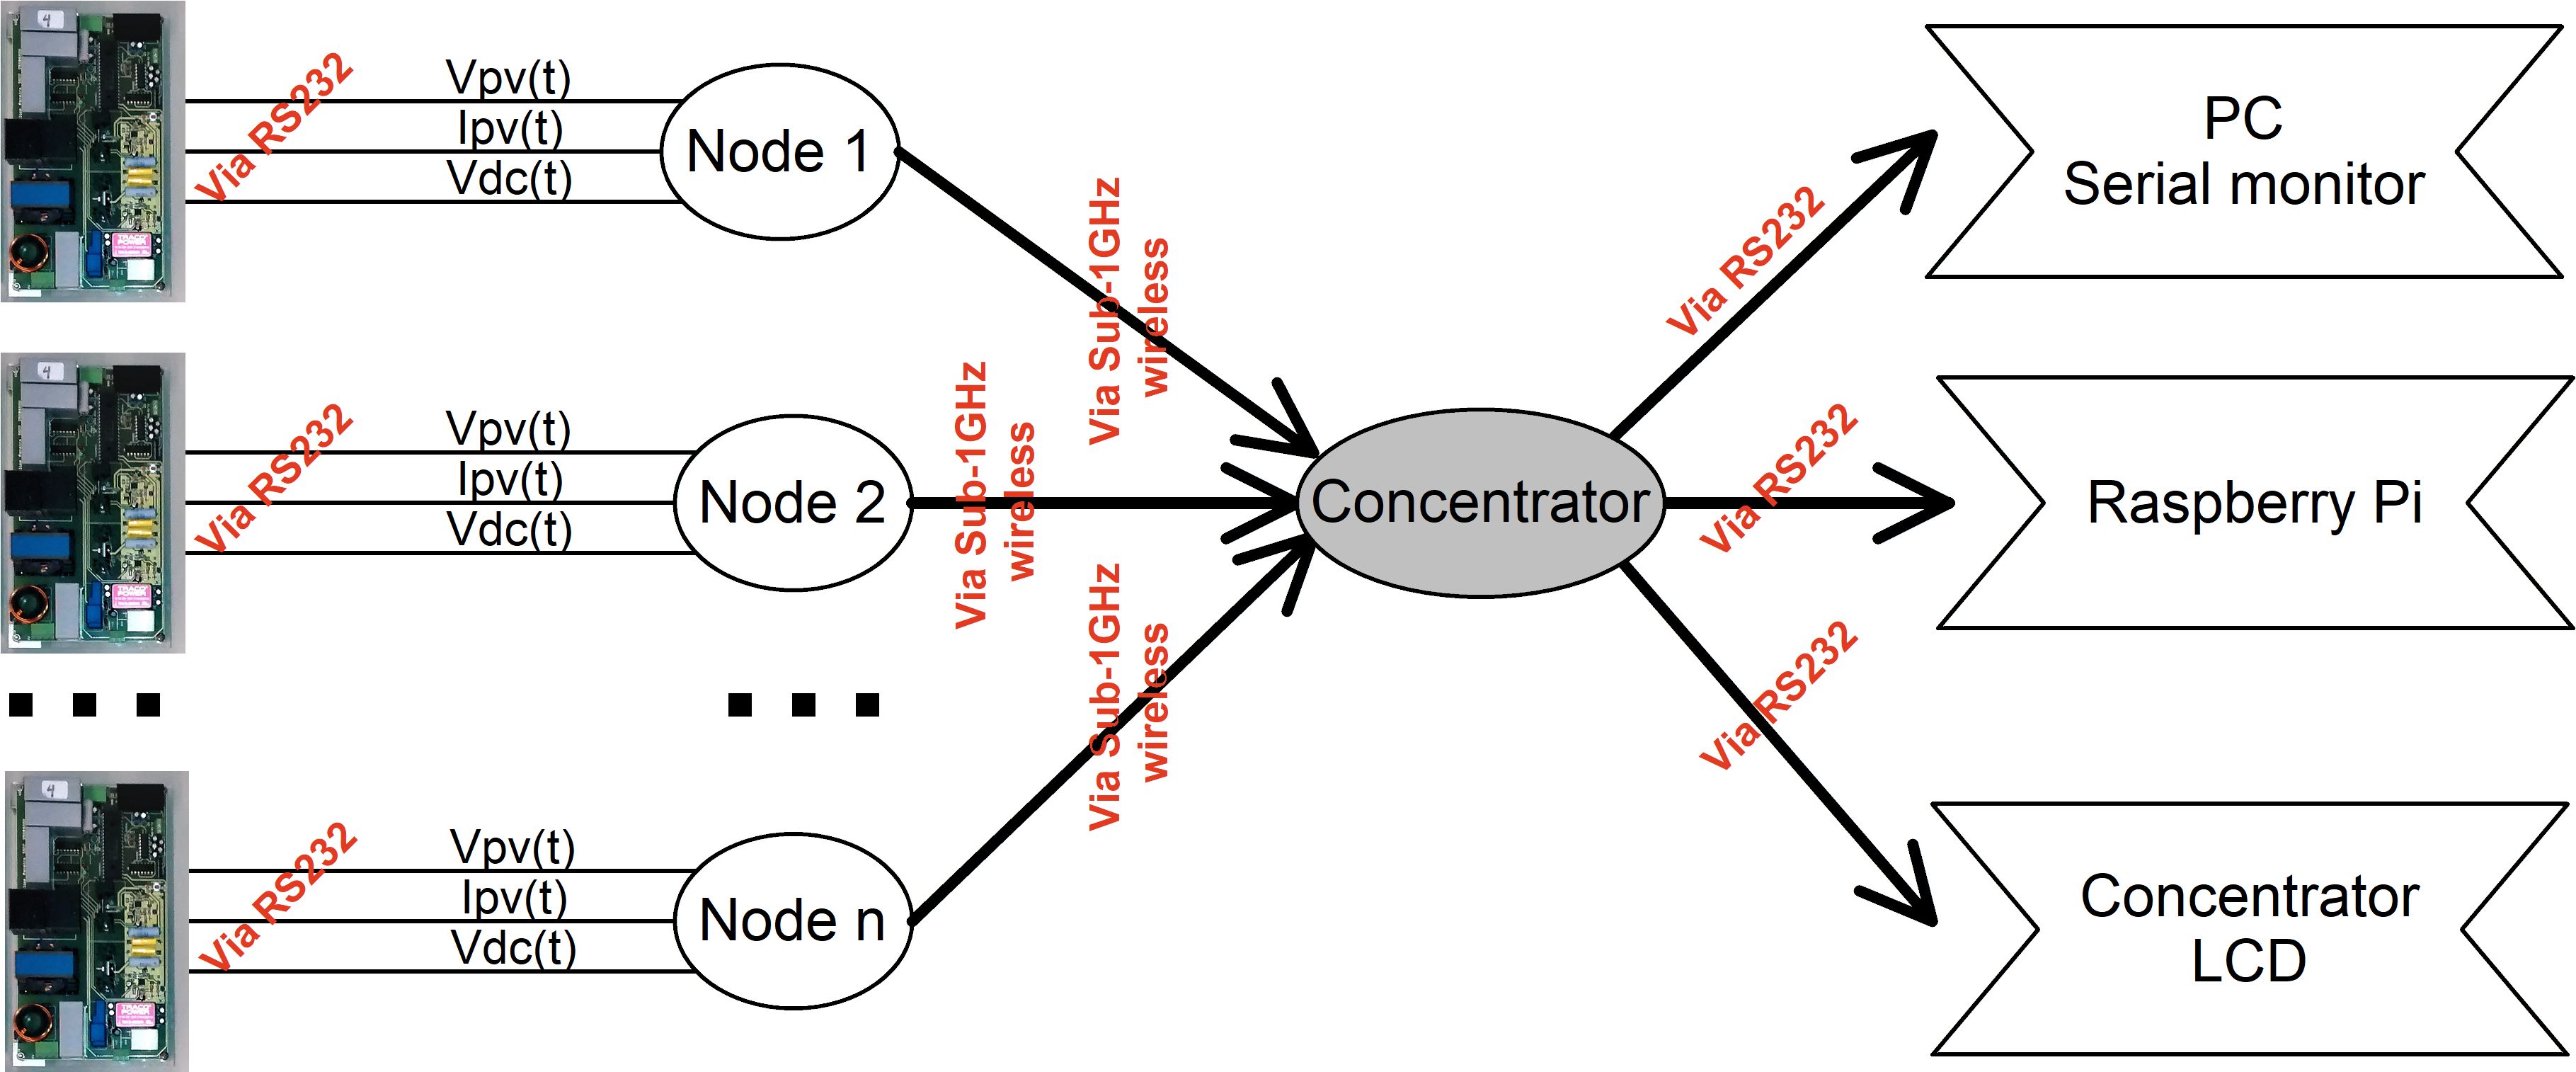
\includegraphics[width=0.9\textwidth,keepaspectratio]{figures/hw}
	\caption{Hardware architecture.}
	\label{fig:3.2.hw}
\end{figure}

The communication interface between node and power converter must support different voltage levels (in particular 3.3V from CC1350 node and 5V from power converter). This way, an electronic board (PCB) was developed to support this constraint. Complementary, this PCB allows a robust mechanical interface between the wireless node and the power converter, without extending the dimensions defined in the SRS. This PCB integration with wireless node and the power converter is presented in the figure \ref{fig:3.2.pcb}.

\begin{figure}[h!]
	\centering
	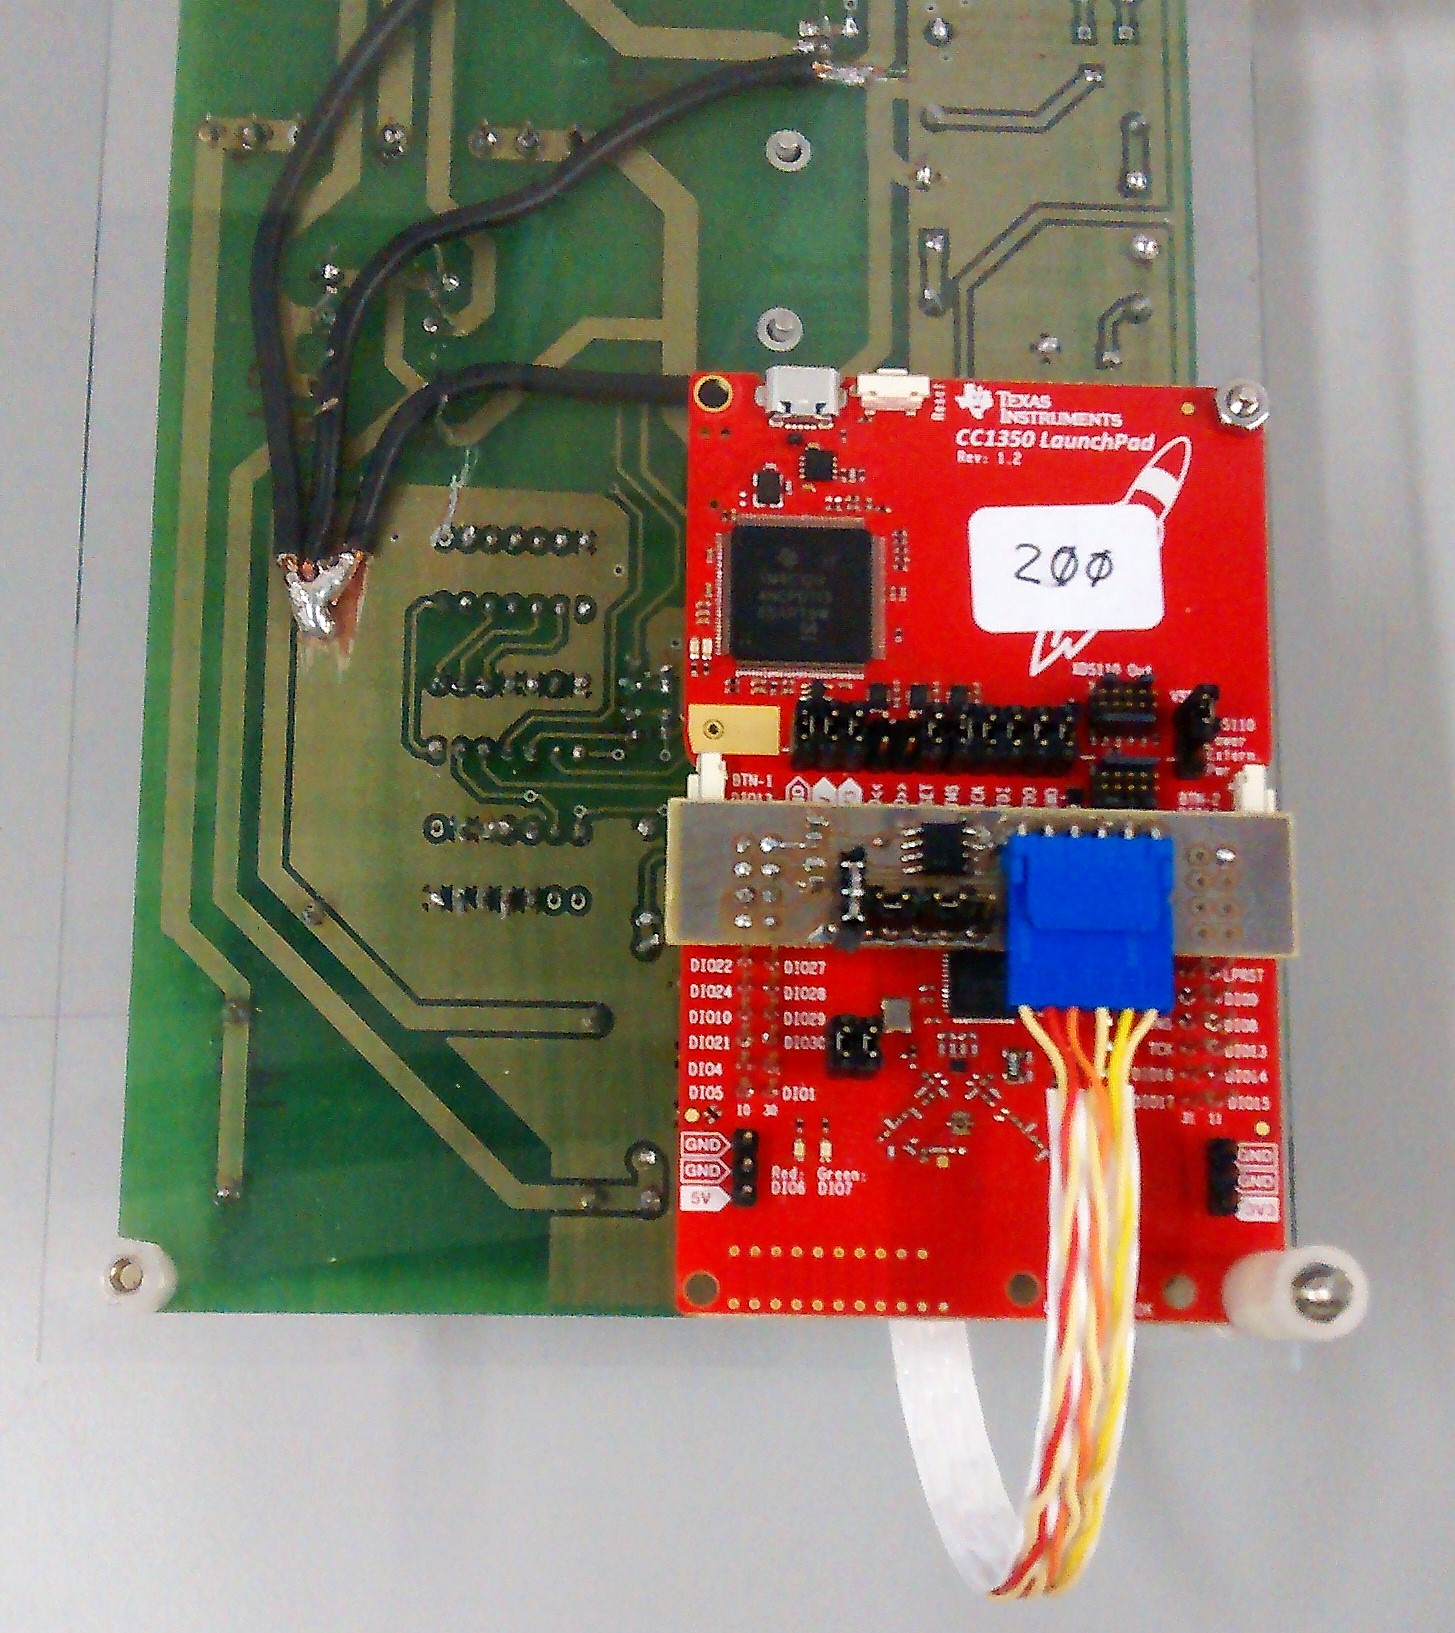
\includegraphics[width=0.4\textwidth,keepaspectratio]{figures/pcb}
	\caption{PCB integration with wireless node and the power converter.}
	\label{fig:3.2.pcb}
\end{figure}

On the concentrator side, the CC1350 development board has available the USB serial communication as well as the LCD as shown in figure \ref{fig:3.2.concentr}.

\begin{figure}[h!]
	\centering
	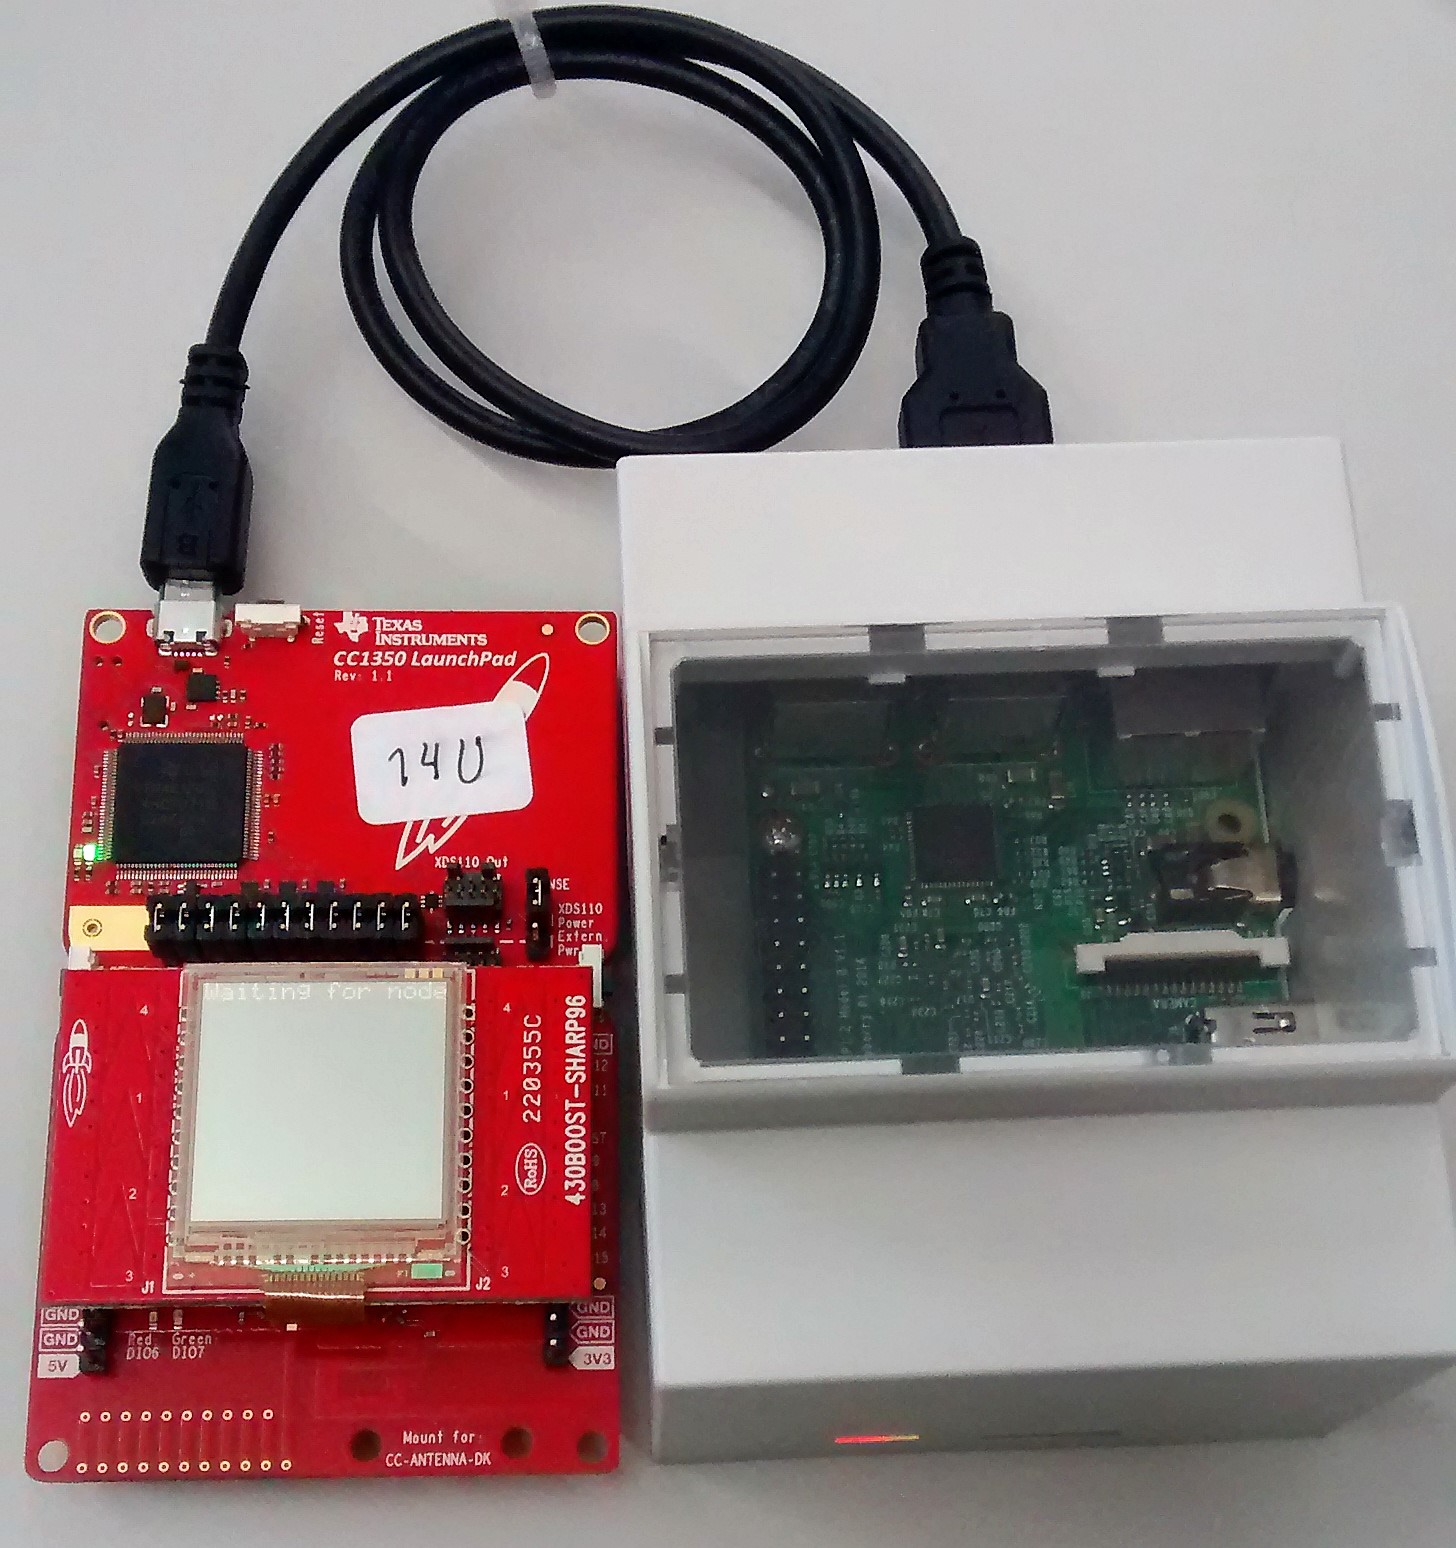
\includegraphics[width=0.5\textwidth,keepaspectratio]{figures/concentr}
	\caption{Concentrator connected to RPI.}
	\label{fig:3.2.concentr}
\end{figure}

\section{Software Architecture}
\label{sec:3.3}
%\lipsum[4-4]

As proposed in the SRS, figure \ref{fig:3.3.domainModel} presents the domain model of the software to be implemented in the concentrator and nodes.

\begin{figure}[h!]
	\centering
	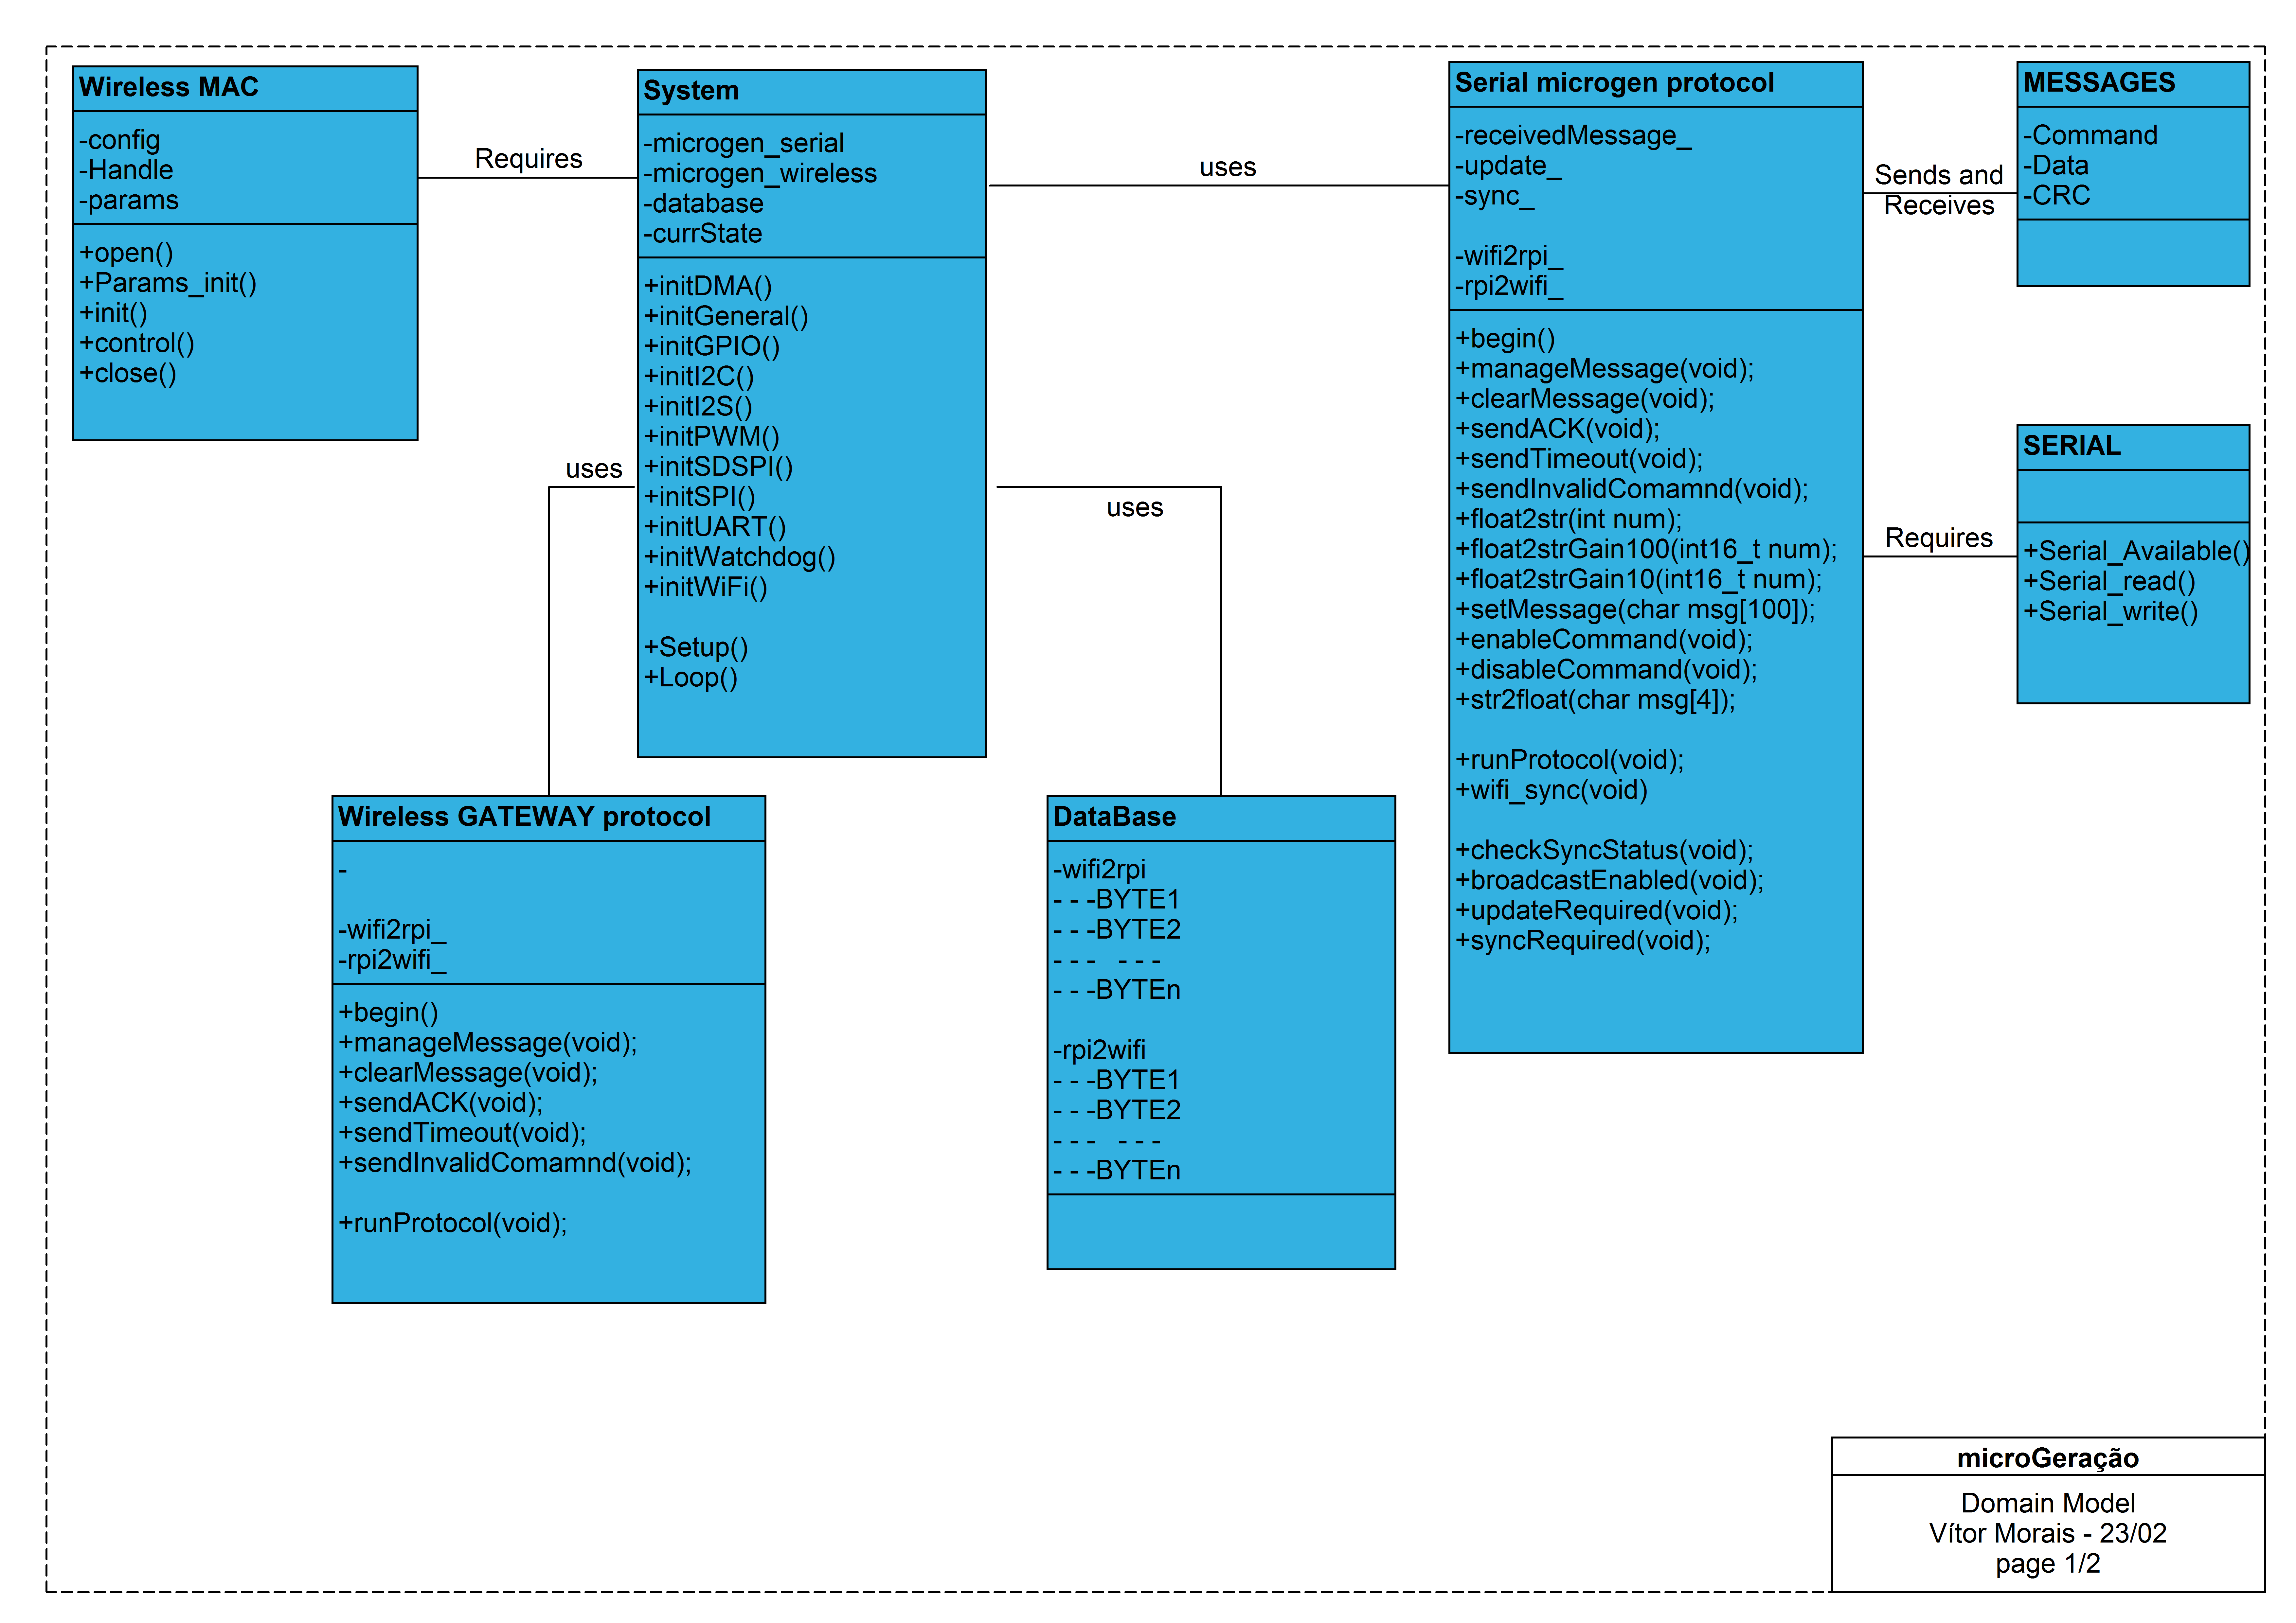
\includegraphics[width=\textwidth,keepaspectratio]{figures/domainModel}
	\caption{Domain Model Diagram.}
	\label{fig:3.3.domainModel}
\end{figure}

The software architecture was based on a proprietary implementation of a WSN by the manufacturer of the CC1350 (Texas Instruments).



\section{Communication results and KPI metrics}
\label{sec:3.4}
\lipsum[4-4]

\section{Discussion of the results}
\label{sec:3.5}
\lipsum[4-4]